\section{Question 8}
    \subsection{\textbf{Specify the Polling Server for this task set. Maximize server utilization, i.e., do the best server you can. Motivate your answer e.g. by a schedulability analysis}}

        The task set will be scheduled with RM. To make sure the task set is schedulable with the extension of a PS, we have to make sure the following statement is true: $U_P + U_S <= (n+1)(2^{\frac{1}{n+1}} - 1)$ where $n$ is the number of tasks in the task set. 
        The following is the given task set:

        \renewcommand{\arraystretch}{1.4}
            \begin{figure}[H]
            \centering
            \begin{minipage}{0.5\textwidth}
                \begin{table}[H]
                \centering
                \begin{tabular}{|l|l|l|}
                    \hline
                    \textbf{Task}   & \textbf{T=D}  & \textbf{C}  \\ \hline
                    A               & 6             & 1           \\ \hline
                    B               & 8             & 2           \\ \hline
                    C               & 12            & 3           \\ \hline
                \end{tabular}
                \end{table}
            \end{minipage}%
            \caption{Task set}
            \label{fig:Q8tasks}
            \end{figure}
        \renewcommand{\arraystretch}{1.0}


        \begin{itemize}
            \item $U_P = \sum_{i=1}^{n} \frac{C_i}{T_i} = \frac{1}{6} + \frac{2}{8} + \frac{3}{12} = \frac{2}{3}$
            \item $\frac{2}{3} + U_S <= (3+1)(2^{\frac{1}{3+1}} - 1) = 0.757$
            \item $U_S <= 0.757 - \frac{2}{3} = 0.09$
        \end{itemize}

        When using the sufficient testing method above, the maximum $U_S$ is $0.09$ to make the task set schedulable with the extension of a PS. A PS which supports this $U_S$ is:
        \begin{itemize}
            \item $C_s = 9ms$
            \item $T_s = 100ms$
        \end{itemize}

        This is not a good solution since the server utilization is very low. We can try to find a better solution by analyzing the trace of the task set. The following figure shows the tracing of the task set with the PS specified above.

        To find a better we have to analyse the trace of the task set. The sak set without the PS is shown in the following figure.

        \begin{figure}[H]
            \centering
            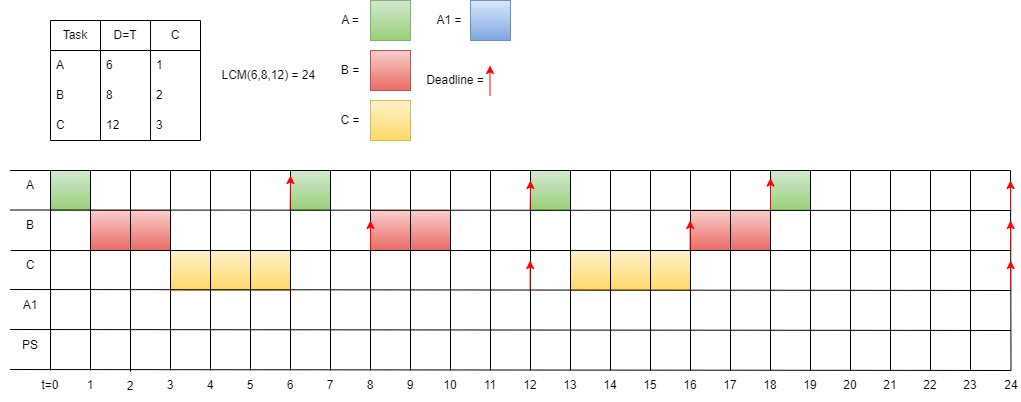
\includegraphics[width=0.8\textwidth]{images/Ass1Q8a.png}
            \caption{Tracing of the task set without PS.}
            \label{fig:Q8Atrace}
        \end{figure}

        In figure \ref{fig:Q8Atrace} we can see that we have a total of 8 time units of no execution. What we can do first is to try to find a PS which can fill all of the empty time units. In that case we get a PS with $T_S = \frac{24}{8} = 3ms$ and $C_S = 1ms$. This gives a server utilization of $U_S = \frac{1}{3}$. Using this server we would fill all empty time units. However, we can see that there is only thee empty time units in the first half of the LCM trace when we would need 4. This means we cannot use a server with $C_S = 1ms$ and $T_S = 3ms$ since other tasks would miss their deadlines. We can the try to reduce the server utilization to $U_S = \frac{1}{4}$. This gives a server with $C_S = 1ms$ and $T_S = 4ms$. This server would only fill 6 of the empty time units, but it might make the task set schedulable. The following figure shows the tracing of the task set with the PS specified above.

        \begin{figure}[H]
            \centering
            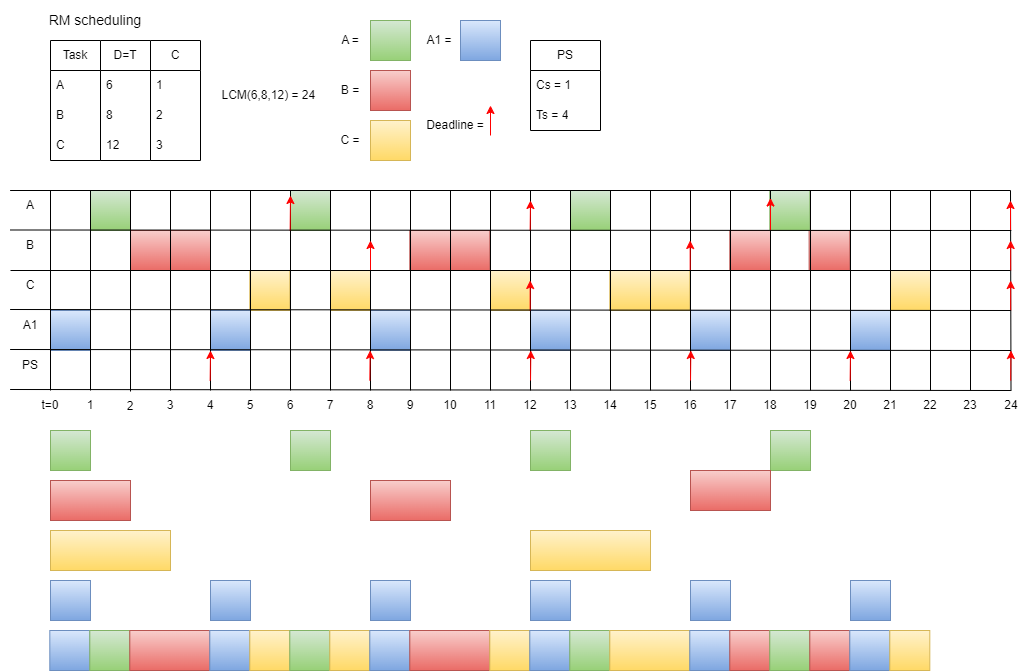
\includegraphics[width=0.8\textwidth]{images/Ass1Q8aPS.png}
            \caption{Tracing of the task set along PS with $C_S = 1ms$ and $T_S = 4ms$.}
            \label{fig:Q8PStrace}
        \end{figure} 

        In figure \ref{fig:Q8PStrace} we can see that the task set is schedulable with the PS specified above. This means that the maximum server utilization is $U_S = \frac{1}{4}$ to make the task set schedulable with the extension of a PS. This is a better solution than the one found using the sufficient testing method since the test is exact and we get a better result.

    \subsection{\textbf{The same question as above, but for Total Bandwidth Server}}
        
        This time the task set will be scheduled using EDF. To make sure the task set is schedulable with the extension of a TBS, we have to make sure the following statement is true: $U_P + U_S <= 1$ where $U_S$ is the processor utilization factor of the TBS. $U_P = \frac{2}{3}$ as before and to make the statement true we have to make sure that $U_S <= 1 - \frac{2}{3} = \frac{1}{3}$. So the maximum $U_S$ is $\frac{1}{3}$ to make the task set schedulable with the extension of a TBS.

    \subsection{\textbf{Soft aperiodic tasks}}

        Assuming the aperiodic tasks enters the TBS system from question b. Aperiodic task A1 enters at $t=4$, $a_{A1} = 4$. This will give A1 a deadline of $4 + \frac{C_{A1}}{U_S} = 4 + \frac{2}{\frac{1}{3}} = 4 + 6 = 10ms$. Task A2 enters at $t=6$, $a_{A2}$. This will give A2 a deadline of $d_{A2} = max(a_{A2}, d_{A2}) + \frac{C_{A2}}{U_S} = 10 + \frac{C_{A2}}{U_S} = 10 + \frac{2}{\frac{1}{3}} = 10 + 6 = 16ms$. The task set and the aperiodic tasks will be scheduled using EDF. If two tasks happen to have the same deadline, the one that arrived earlier will be executed first. The following figure shows the tracing of the task set with the soft aperiodic tasks A1 and A2.

        \begin{figure}[H]
            \centering
            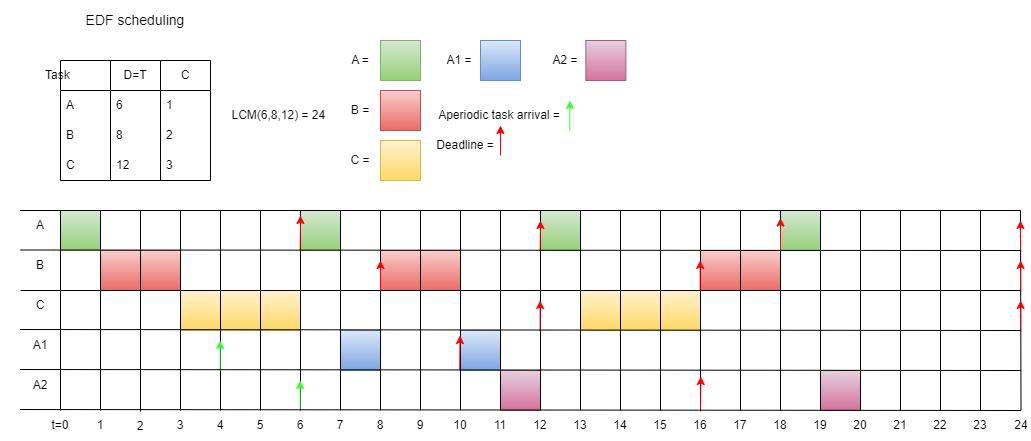
\includegraphics[width=0.8\textwidth]{images/Ass1Q8c.png}
            \caption{Tracing of the task set with soft aperiodic tasks A1 and A2.}
            \label{fig:Q8Ctrace}
        \end{figure}